\documentclass[twoside,zh,watermark,final]{config/thesis}  % draft mode (default)
%\documentclass[review]{thesis}  % review mode (show contents & reference only)
%\documentclass[watermark,final]{thesis}  % final mode (version for library)

%-------------------------------------------------------------------------------
% Package Loading
%-------------------------------------------------------------------------------

\usepackage{multirow}     % for multi-row table
\usepackage{booktabs}     % table style used in books

%-------------------------------------------------------------------------------
% Configuration
%-------------------------------------------------------------------------------

% 填寫題目, 作者, 指導教授, 學校, 系所, 日期等資訊
% Title
\title{Thesis title}
\titlezh{中文論文標題}

% Author
\author{Example Name}
\authorzh{中文名}

% Advisor
\advisor{Huan Chen}
\advisorzh{陳 \quad 煥}

% First co-advisor (Leave {} empty if you don't have a co-advisor)
% \coadvisorA{English Name}
% \coadvisorAzh{中文名}

% Second co-advisor (Leave {} empty if you don't have a second co-advisor)
% \coadvisorB{}
% \coadvisorBzh{}

% Field
\field{Computer Science}

% Institute
\institute{Institute of Computer Science and Engineering}
\institutezh{資訊科學與工程學系}

% College
\college{College of Electrical Engineering and Computer Science}

% University
\university{National Chung Hsing University}
\universityzh{國立中興大學}

% Location
\location{Taichung, Taiwan}

% Date of final submission
\degreemonth{June}
\degreeyear{2023}
\degreeyearzh{中 華 民 國 一 百 一 十 一 年 八 月}

% Watermark
\watermark{config/nchu_logo.jpg}

% 修改 thesis.cls 的預設字型
%-------------------------------------------------------------------------------
% Chinese Font Settings
%
%   These macros are used to change the default Chinese fonts (see below) used
% by thesis.cls. Please leave {} empty if you want to use the default settings
% and make sure that you have added '-shell-escape' option when using xetex to
% compile tex files, i.e. xetex compiling commands should run something like:
%
%     xelatex -synctex=1 -shell-escape -interaction=nonstopmode %.tex
%
% (default Chinese font settings)
%   Windows              Linux                        Mac OS X
% * 標楷體 (DFKai-SB)    AR PL 中楷 (AR PL UKai TW)   楷體-繁 (Kaiti TC Regular)
% @ 新細明體 (PMingLiU)  AR PL 明體 (AR PL UMing TW)  儷宋 Pro (LiSong Pro)
%
% * fontname --> 預設中文本文字型 (serif)
% @ fontname --> 預設中文明體字型 (sans-serif, 使用於封面頁)
%-------------------------------------------------------------------------------

% main (serif) Chinese font, leave {} empty to enable default font setting
\mainfontzh{AR PL UKai TW}

% sans-serif Chinese font, leave {} empty to enable default font setting
\sansfontzh{AR PL UKai TW}

%-------------------------------------------------------------------------------
% English Font Settings
%
%   These macros are used to change the default English fonts (see below) used
% by thesis.cls. Please leave {} empty if you want to use the default settings.
%
% (default English font settings)
% main font       --> Times New Roman (for all platforms)
% sans-serif font --> Arial           (for all platforms)
%-------------------------------------------------------------------------------

% main font for English, leave {} empty if you want to use default font setting
\mainfont{FreeSerif}

% sans-serif font for English, leave {} empty if you want to use default setting
\sansfont{FreeSerif}



\begin{document}

% Show repeated author names in bibliography when using IEEEtran.bst
% Comment out this line if you don't set IEEEtran in \bibliographystyle{}
\bstctlcite{IEEEexample:BSTcontrol}

% Generate cover, title, authorization, approval and copyright pages
\maketitle

% Equation numbering without chapter number
\counterwithout{equation}{chapter}

% Indent two character
\setlength{\parindent}{2em}

%-------------------------------------------------------------------------------
% Acknowledgement
%-------------------------------------------------------------------------------

% 誌謝
%\input{ack/ack}

% 題獻頁 (Only shown in the final mode of a PhD dissertation)
%\input{ack/dedication}

%-------------------------------------------------------------------------------
% Abstract
%-------------------------------------------------------------------------------

% 中文摘要
\begin{abstractzh}
無線感測網路(Wireless Sensor Networks,簡稱 WSN)在現代科技中扮演著越來越重要的角色,但它們面臨著許多挑戰。其中一個主要的挑戰是如何有效地處理數據,因為傳輸過程中可能發生許多錯誤和丟包。解決這個問題的一種方法是利用元學習(Meta Learning)。元學習是一種學習如何學習的方法,它通常被應用於機器學習領域。在 WSN 中,元學習可以幫助系統學習如何在不同的網絡環境中自適應地處理數據。通過利用元學習的技術,WSN 可以根據網絡環境自動調整自己的參數和策略,提高整個系統的效率和準確性。具體來說,元學習可以幫助 WSN 實現以下目標:
在不同的網絡環境中自適應地調整數據處理策略,從而提高系統的效率和準確性。
自動調整系統的參數,從而適應不同的網絡場景和任務。學習如何優化網絡拓撲結構,從而提高網絡的穩定性和可靠性。
總之,元學習可以幫助 WSN 自動學習和優化系統的性能,從而解決數據處理方面的問題。這將有助於提高 WSN 的效率、可靠性和應用範圍,推動其在現代科技中的應用。

\providecommand{\keywords}[1]
{
\small  
\textbf{{關鍵字:}} #1
}
\keywords{自適應元學習、元學習、無線感測網路}
\end{abstractzh}

% 英文摘要
\begin{abstract}%
Wireless Sensor Networks (WSNs) play an increasingly important role in modern technology, but they face many challenges. One major challenge is how to efficiently handle data, as errors and packet loss can occur during transmission. One solution to this problem is to utilize metalearning.
Metalearning is a method of learning how to learn and is often applied in the field of machine learning. In WSNs, metalearning can help the system learn how to adaptively process data in different network environments. By leveraging metalearning techniques, WSNs can automatically adjust their parameters and strategies based on the network environment, improving the efficiency and accuracy of the entire system.
Specifically, metalearning can help WSNs achieve the following goals:
Adaptively adjust data processing strategies in different network environments to improve system efficiency and accuracy.
Automatically adjust system parameters to adapt to different network scenarios and tasks.
Learn how to optimize network topology structures to improve network stability and reliability.
In summary, metalearning can help WSNs automatically learn and optimize system performance, thereby addressing data processing issues. This will help improve the efficiency, reliability, and application range of WSNs, promoting their use in modern technology.

\providecommand{\keywords}[1]
    {
    \small  
    \textbf{{Keywords: }} #1
    }
    \keywords{metalearning, WSNs, adaptively}
\end{abstract}

%-------------------------------------------------------------------------------
% 目錄
%-------------------------------------------------------------------------------

% Generate 'Table of Contents', 'List of Figures', and 'List of Tables', and
% Set page numbering to 'arabic'
\maketocs

%-------------------------------------------------------------------------------
% Contents
%-------------------------------------------------------------------------------

% Set page numbering to 'arabic' (1, 2, 3, ...)
\mainmatter

% 內文, 請依照章節順序擺放
\chapter{緒論}
\label{chapter:intro}
\section{簡介}
% %IoT的重要性及地位
% 巨量資料所隱含的價值被挖掘後,物聯網受重視的程度也隨之提昇。其概念是串連人們身邊隨處可見的裝置及服務,整合原本分散的應用使其發揮更高的價值。
% %IoT的困難
% 嶄新的商業模式及應用需要分佈大量的感測器以提高覆蓋率,這使得整個物聯網系統的安全性、可靠度、負載率、產出及連接性都受到巨大的挑戰。對於一個延遲靈敏度高的服務而言,建構一
% 個高可靠度及效能表現穩定的系統將直接影響其服務的品質。

%Fog computing的特性及好處
霧運算繼承並且擴展雲端運算的特性及優勢,包含低延遲、分散式架構、機動性,上述特性使其能支援大量的感測器、無線傳輸存取及即時串流服務 \cite{bonomi_2012}。其優異的特性適合建構
高效的物聯網相關應用。
%Fog computing的必要性
例如智慧電網就需要建置大量的智慧電錶作為感測器,並且即時監測、回傳用電資訊至伺服器以進行下一步的運算 \cite{yi_2015}。若智慧電網系統是以霧運算架構為其基本建置結構,整體智慧
電網就可視為許多小型智慧電網群集的集合。用電資料將區域性的運算並即時回傳,需要整合性的做大量運算時才會回傳至運算中心以大型伺服器運算。此舉降低集中式伺服器的負載,同時享有
靈活調度運算資源的好處。

%Fog computing的分配是個問題
享有霧運算系統帶來的好處之前,要先解決其階層型的分散式架構的配置問題。配置伺服器將直接影響整體霧運算系統完成後的效能以及成本。霧運算伺服器將依據其配置位置調整服務,例如針
對區域性的需求客製化該區伺服器提供的應用,並在各霧運算群集中配置足夠的運算資源以就近服務終端使用者 \cite{luan_2015}。
%此分配問題是NP-hard問題
霧運算遇到的配置問題為如何找到一個資源配置的方案,使得各資源間的連線達成低延遲、低成本、高覆蓋率且能滿足各階層的運算需求量。此類型問題可被轉變為度受限最小生成樹
(degree-constrained minimum-spanning tree; DCMST)問題 \cite{kim_2015}。而在兩個以上的度限制下尋找DCMST是已知的NP-hard問題 \cite{narula_1980},故霧運算分配問題也是NP-hard
問題。

%NP-hard就用啟發式解決
目前NP-hard問題還沒有有效的方法可以在合理的時間內找到最佳解。所以此類問題通常會轉而在合理時間內,最大程度的找尋近似最佳解。相較於最佳化演算法或疊代法,超啟發式
(metaheristic)演算法雖然無法保證提供全域最佳解,但保證能在運算時間有限的情況下,對最佳化問題提供足夠好的區域最佳解。
\\
\\

\section{研究動機}
%應用到霧運算分配問題會有些問題
霧運算系統分配問題應用於智慧電網、工業4.0等環境中,因應大量的終端使用者,需要建置非常大量的感測器、邊緣運算伺服器以及霧運算伺服器。而運算產生的巨量資料也需要在各霧運算群
集中分配閘道器。此環境下的資源配置就形成一個巨大解空間的最佳化問題。
%啟發式演算法能解決小型的分配問題,針對大解空間的問題做不好
超啟發式演算法之所以無法保證提供全域最佳解的原因在於其尋優策略的特性。其核心想法是隨機產生一或多組初始解,藉由疊代從初始解開始探索解空間。而每次疊代都會保留原本解的部份特
徵,期望此特徵是構成最佳解的子特徵。但若保留下的特徵是區域最佳解的特徵將使得最終結果落到區域最佳解的可能性上升。在解空間較小的分配問題上,區域最佳解的數量較少,尋優過程中
也較容易均勻的探索整個解空間。傳統的超啟發式演算法如基因演算法(genetic algorithm; GA) \cite{holland_1962}、模擬退火(simulated annealing; SA) \cite{kirkpatrick_1983}、粒
子群最佳化演算法(particle swarm optimization; PSO) \cite{kennedy_1995}等都能提供良好的尋優效果。針對解空間大的最佳化問題,傳統超啟發式演算法會因為區域最佳解數量龐大抑或
沒有均勻的在解空間內尋優,而無法在合理的時間內提供夠好的區域最佳解。

% 即便某些演算法有一定的機率透過暫時接受較差解的方式試圖跳出該區域最佳解,但仍舊無法解決均勻的搜尋整個解空間的問題。若以跳出區域最佳解的方式面對龐大數量的區域最佳解,也只
% 會使得疊代次數增加。

%大解空間的問題有幾種策略
超啟發式演算法面臨此問題的策略主要都是增加搜尋多樣性。例如增加候選解數量以提高每次疊代可以搜尋區域最佳解的數量,並藉由交換各區域最佳解的特徵,嘗試組合出更加優秀的解。雖然
這種作法的確提昇解的品質,但在交換各區域最佳解的特徵的同時,搜尋多樣性的特性也隨之消失。各候選解容易漸漸朝向同樣區域尋優,疊代後期容易花費大量計算資源在重複的區域而無法進
一步得到新的最佳解。
%SE可以對大解空間做得不錯
Tsai \cite{tsai_2015}提出的搜尋經濟學演算法(search economics)針對上述問題發展一套基於切割解空間的框架,在切割的子解空間內依據其潛力投放搜尋資源。其主要目標是增加搜尋多
樣性且避免後期搜尋資源的浪費。不論在疊代前期抑或後期,搜尋資源將藉由該框架的分配而均勻的在分割後的解空間中搜尋。
\\
\\
\\
% 本論文將以擅長在大型解空間尋優的搜尋經濟學演算法解決此一配置問題。
\section{貢獻}
本論文提出一個基於搜尋經濟學演算法的霧運算系統配置演算法。在運算資源需求驟增的物聯網環境中,利用搜尋經濟演算法不易落入區域最佳解的特性解決配置問題。本論文主要貢獻分為以下
三點:
\begin{enumerate}[\hspace{2em}(\xCJKnumber{\arabic{enumi}})]
    \item 將搜尋經濟學演算法切割解空間的機制融合霧運算系統階層型的分散式架構的特性,對解空間進行有意義的切割。
    \item 基於搜尋經濟學演算法定義的兩種不同搜尋資源制定兼容貪婪性及搜尋多樣性的搜尋策略。
    \item 新增的貿易運算子改良搜尋資源在解空間中探索的機制,針對尚未收斂的區域加強搜尋以增進搜尋效率。
\end{enumerate}
以上三點改良使搜尋經濟學演算法在霧運算系統配置問題中能夠加強其搜尋廣度、深度、持續性及搜尋效率。相較於基於規則的最佳優先演算法、早期提出的基因演算法以及近期改良的離散猴群
基因演算法、離散猴群演算法,本論文在衡量成本、覆蓋率、傳輸延遲以及服務需求的綜合評量指標獲得更佳的結果。

\section{論文架構}
如圖 \ref{fig:thesis-arch},第二章首先整理相關問題定義,將實際的霧運算系統配置問題釐清。量化在霧運算系統內影響配置結果的重要指標,並定義實際計算方法。接著說明一個基於規則的演算法、一個早期的最佳化演
算法以及兩個近年針對類似分配問題的改良型演算法。詳細探討上述演算法原理以及在複雜解空間下的缺點。第三章將針對搜尋經濟學演算法深入探討,將分別介紹演算法中重要的運算子運作原
理及特性。對於改良的機制進行步驟及原理說明。第四章介紹實驗環境、測試資料集產生方法及資料集特性。演算法參數調整過程、實驗結果呈現及說明。第五章總結本篇論文結果,探討不足之
處作為未來改良方向。
\begin{figure}[H]
    \centering
    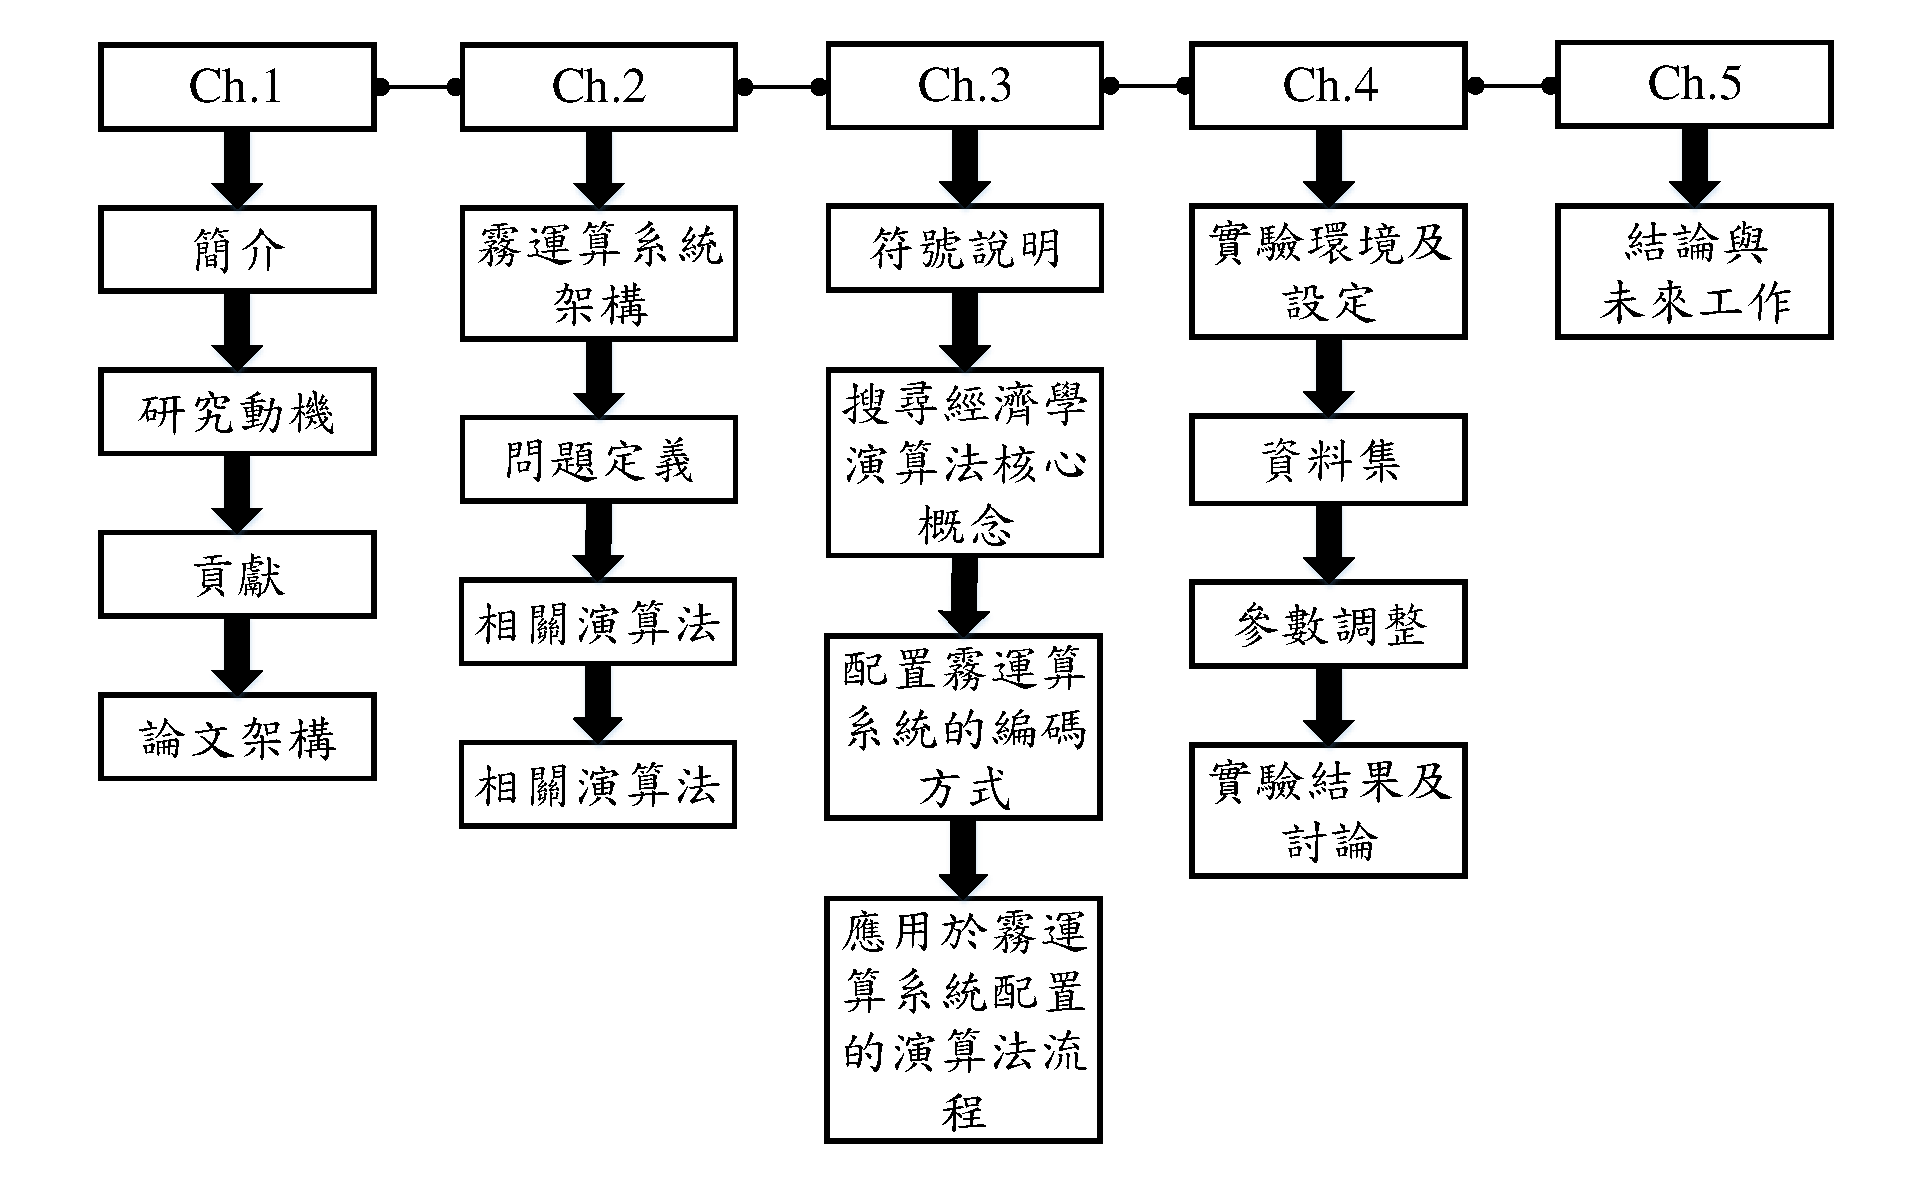
\includegraphics[height=!,width=1\linewidth,keepaspectratio=ture]
    {figures/thesis_arch}
    \caption[論文架構圖]{\normalsize 論文架構圖}
    \label{fig:thesis-arch}
\end{figure}


\chapter{背景知識與相關研究}
\label{chapter:rtl-work}
\section{霧運算系統架構}
\label{section:architechture}


\section{問題定義}
\label{section:problem-definition}
%分配fog computing server會影響到的項目
本研究基於Lin \cite{lin_2018}針對智慧物流中心配置霧運算系統的問題定義衡量配置演算法。該研究基於上述霧運算架構特性,定義衡量霧運算架構的目標函式如下:
\begin{flalign}
    \label{equa:objective}
    &f = C_{l} + C_s + P,&
\end{flalign}
其中$C_{ij}$為衡量節點$i$及節點$j$的連線成本,$C_s$為所有伺服器的建置成本,$P$為懲罰成本。計算方式分別如下:
\begin{flalign}
    \label{equa:link-cost}
    &C_l = c_f \sum_{(i,j)\in\{s\}\times\Omega_G\cup\Omega_G\times\Omega_F\cup\Omega_F\times\Omega_E} x_{ij} \cdot d_{ij},&\\
    \label{equa:server-cost}
    &C_s = c_G \sum_{m\in\Omega_G}g_m + c_F \sum_{n\in\Omega_F} f_n + c_E \sum_{t\in\Omega_E} q_t,&\\
    \label{equa:penalty-cost}
    &P = \kappa \cdot (\eta_{\text{link}} + \eta_{\text{demand}} + \eta_{\text{latency}} + \eta_{\text{cover}} + \eta_{\text{capacity}}),&
\end{flalign}
公式 \ref{equa:link-cost}中,$c_f$為配置一單位光纖的價格,$x_{ij}$與$d_{ij}$分別為第$i$個節點與第$j$個節點間有無配置光纖的二進制數及其距離。若節點$i$、$j$間有連線需求,則
依照距離計算成本。公式 \ref{equa:server-cost}的$c_G$、$c_F$及$c_E$分別為安裝一個閘道器、霧伺服器及邊緣伺服器的成本。$g_m$、$f_n$及$q_t$則分別代表候選位置有無安裝閘道器、霧
伺服器及邊緣伺服器的二進制數。若有配置裝置則按照數量計算所有已配置伺服器的成本。在實際的霧運算系統中,有些限制是無法在解空間中定義並且從解空間中分離的。這些限制會以增加目標值
(objective value)的方式避免,有許多項目超出限制的霧運算系統將獲得極高的目標值,增加目標值的方式如公式 \ref{equa:penalty-cost}。$\kappa$為懲罰成本,
$\eta_{\text{link}}$、$\eta_{\text{demand}}$、$\eta_{\text{latency}}$、$\eta_{\text{cover}}$及$\eta_{\text{capacity}}$是在統計一個配置完的的霧運算系統有多少項目是超出限制
的。計算方式分別如下:
\begin{enumerate}[\hspace{2em}(\xCJKnumber{\arabic{enumi}})]
    \item 連線限制$\eta_{\text{link}}$:計算有多少的使用者或伺服器沒有被服務,即任意使用者、邊緣伺服器或霧伺服器$i$沒有分別被配置到邊緣伺服器、霧伺服器或閘道器$j$的情況是不被允許的:
    \begin{flalign}
        \label{equa:eta-link}
        &\eta_{\text{link}} \leftarrow \eta_{\text{link}}+1\text{,\quad if } x_{ij}=0,&
    \end{flalign}
    $x_{ij}$為代表裝置$i$及裝置$j$間有無配置線路的布林值。
    \item 服務限制$\eta_{\text{demand}}$:限制著每個伺服器能夠處理的服務量。每個使用者會有各自產生的基本服務需求量$r_A$,此服務需求量會由服務該使用者的邊緣伺服器接收。而
    霧伺服器及閘道器也將分別接收其服務的邊緣伺服器及霧伺服器的服務需求。邊緣伺服器$t$、霧伺服器$n$及閘道器$m$都有其能負荷的最大處理需求量$H^E_t$、$H^F_n$及$H^G_m$。對於任
    意伺服器或閘道器$j$,從低其一階的裝置$i$接收的服務需求量超出負荷是不被允許的:
    \begin{flalign}
        \label{equa:eta-demand}
        &\eta_{\text{demand}} \leftarrow \eta_{\text{demand}}+1\text{,\quad if } \sum_{k\in\Omega_i}r_i\cdot x_{jk} > H^E_j.&
    \end{flalign}
    \item 延遲限制$\eta_{\text{latency}}$:每個伺服器$i$的延遲時間是其所有服務的裝置$j$所造成延遲時間的總和,是由被服務裝置所產生的資料量$L_j$及其資料傳輸率$\gamma_j$而
    得。此項限制任意被配置伺服器$i$與其所有服務的裝置$j$的延遲率和大於延遲時間門檻$D_{ij}$:
    \begin{flalign}
        \label{equa:eta-latency}
        &\eta_{\text{latency}} \leftarrow \eta_{\text{latency}}+1 \text{,\quad if } \sum_{j}{L_j\over(x_{ij}\cdot\gamma_j)}>D_{ij}.&
    \end{flalign}
    \item 覆蓋限制$\eta_{\text{cover}}$:每個使用者附近至少要配置一個邊緣伺服器。對於任意使用者$k$,服務該使用者的邊緣伺服器$t$距離$d_{tk}$不得大於邊緣伺服器服務的半徑$R_E$:
    \begin{flalign}
        \label{equa:eta-cover}
        &\eta_{\text{cover}} \leftarrow \eta_{\text{cover}}+1 \text{,\quad if } x_{tk}\cdot d_{tk} > {R_E\over2}.&
    \end{flalign}
    \item 容量限制$\eta_{\text{capacity}}$:邊緣伺服器、霧伺服器及閘道器分別能容納的最大裝置容量分別為$N_E$、$N_F$及$N_G$。$\eta_{\text{capacity}}$計算任意超出裝置自身最
    大容量的伺服器$j$的數量:
    \begin{flalign}
        \label{equa:eta-capacity}
        &\eta_{\text{capacity}} \leftarrow \eta_{\text{capacity}}+1 \text{,\quad if } \sum_{k\in\Omega_i}x_{jk}\leq N_j.&
    \end{flalign}
\end{enumerate}

目標值將建置整個系統的成本、服務品質、延遲率及效能等考量在內,並藉由懲罰目標值避免伺服器超出負荷、斷線、高延遲等現象。例如圖 \ref{fig:objective}中左邊的範例,配置1個閘道器、1個霧伺服器、
2個邊緣伺服器及8單位的光纖。假設邊緣伺服器最多能夠服務3個使用者,編號(a)的邊緣伺服器服務5個使用者($\eta_{\text{capacity}} = 1$)、且未連線到任何霧伺服器($\eta_{\text{link}} = 1$)
,沒有違反其餘限制項目($\eta_{\text{demand}} = \eta_{\text{latency}} = \eta_{\text{cover}} = 0$),該配置的目標值為$c_G + c_F + 2c_E + 8c_f + 2\kappa$。若能夠將
配置改為右邊的範例,則目標值將降為$c_G + c_F + 2c_E + 9c_f$。在目標函數所形成的解空間中尋找到的最佳解將能以最低成本建置低延遲、高覆蓋率、在合理的伺服器負載下建置所有使用者
都能得到運算資源的霧運算系統。




\subsection{離散猴群基因演算法}
\label{section:dmga}




\section{總結}
...
\chapter{方法}
\label{chapter:method}
\section{符號說明}
\begin{table}[h]
    \small
    \centering
    % \caption{SEFSD與各演算法差異百分比}
    %     \newcommand{\xc}[1]{\multicolumn{1}{c}{#1}}
    %     \newcommand{\z}{\phantom{zzz}}
    %     \newcommand{\za}{\phantom{zz}}
    \begin{tabular}{lll}
        \centering
        符號        &   &代表意義     \\
        $k$         &   &區域的數量。 \\
        $r_i$       &   &第$i$個區域。 \\
        $R$         &   &區域的集合,$R=\{r_1, r_2, \dots, r_k\}$。 \\
        $m$         &   &搜尋者的數量。 \\
        $s^i_j$     &   &投資區域$i$的搜尋者$j$ \\
        $S$         &   &搜尋者的集合,$S=\{s_1, s_2, \dots, s_m\}$。 \\
        $n$         &   &區域內候選商品的數量。 \\
        $g^i_l$     &   &屬於第$i$個區域的第$l$個商品。 \\
        $G^i$       &   &屬於第$i$個區域的商品所形成的集合,$G^i=\{g^i_1, g^i_2, \dots, g^i_n\}$。 \\
        $t^a_i$     &   &區域$i$連續被投資的疊代數。 \\
        $t^b_i$     &   &區域$i$連續未被投資的疊代數。 \\
        $\mu_i$     &   &區域$i$連續被投資比率。 \\
        $\nu_i$     &   &投資區域$i$的投資者平均獲得的目標值。 \\
        $\rho_i$    &   &屬於第$i$個區域的商品平均獲得的目標值。 \\
        $E_i$       &   &區域$i$的期望值。 \\
        $E'_i$      &   &未收斂區域$i$調整後的期望值。 \\
        $o$         &   &參賽者數量。 \\
        $\gamma$    &   &貿易調整未收斂區域期望值的權重參數。 \\
        $t$         &   &疊代次數。 \\
        $d$         &   &擁有最佳目標值的解。 \\
    \end{tabular}
    \label{table:percentage}
    \end{table}

\chapter{實驗結果與討論}
\label{chapter:exp}
\section{實驗環境及設定}
本研究於一台配有兩顆型號為Intel Xeon Silver 4110 (2.1GHz, 11 MB cache, 8 cores)的CPU、16 GB 記憶體及搭載作業系統 Ubuntu 18.04 LTS 的工作站進行實驗。實驗程式碼是以 C++ 撰
寫,編譯器為 gcc 7.4.0。實驗將比較本研究所提之基於搜尋經濟學演算法的霧運算系統配置方法與基於規則的最佳優先演算法(top first) \cite{li_2018}、早期的啟發式演算法——基因演算
法 \cite{holland_1962}及兩個近期的研究分別為基於離散蝙蝠演算法的工作配置演算法 \cite{mishra_2018}及解霧運算系統配置的離散猴群基因演算法 \cite{lin_2018}。基於規則的最佳優先演
算法在策略上最為貪婪,由於 NP-hard 問題無法與窮舉法做比較,故本研究選擇此類有規則限定的疊代演算法。最佳優先演算法優先分配負荷最重的伺服器,在理想情況下(即所有使用者都非
常集中且其附近都有數量足夠的伺服器候選配置地點),其能夠將霧運算系統配置最佳化。基因演算法則是早期最具代表性的超啟發式演算法,已有許多研究將其應用於各種不同性質的配置問題
中,且達到不錯的效果。較近期研究的離散蝙蝠演算法應用於工作配置問題所解決的問題解空間與本研究問題定義都屬於複雜解空間,此實驗將其改實作於霧運算系統配置問題上並比較本研究提
出方法與其在複雜解空間的成效。離散猴群基因演算法是解決霧運算系統配置問題的當前最新演算法,其研究中僅應用於一個空間大小$200m \times 180m$的物流中心,閘道器、霧伺服器、邊緣
伺服器候選位置數量及使用者數量分別為$3$、$15$、$70$及$500$個。本實驗將其應用在閘道器、霧伺服器、邊緣伺服器及使用者數量都更多的複雜資料集中,比較本研究所提配置法與原本即為
霧運算系統配置演算法的效果。
\chapter{結論與未來工作}
\label{chapter:conclusion}
本研究將擅長解決複雜解空間問題的搜尋經濟學演算法應用於霧運算系統的伺服器配置上,解決原本需要考量成本、可連線裝置數量、伺服器工作處理量、延遲時間、覆蓋率及伺服器服務容量互相影響所形成的複雜問題。基於霧
運算系統階層式分散的架構改良配置演算法,結合搜尋經濟學演算法原本切割解空間的作法及霧運算系統配置受到閘道器配置數量影響的特性,發展出具有依據閘道器數量切割並衡量解空間潛力的伺服器配置演算法。在基於閘道
器數量所切割的解空間中,分配可全域移動的搜尋者及固定區域的商品達成全域的貪婪搜尋及區域的多樣搜尋。整體搜尋方向也可因應不同的資料集所產生的特性做策略上的調整,調整參數更細分為對目標值貪婪的商品數量、對
潛力區域貪婪的參賽者數量、對局部增加多樣性的區域數量以及全域多樣性的搜尋者數量。此種搜尋策略大幅度的提升配置演算法整體投入搜尋資源的效率,避免浪費搜尋資源在已搜尋過的區域或是局部沒有潛力的區域。利用區
域投資而得來的全域新解及被投資產生的區域新解計算區域期望值,有效的將資源利用在尚未開發或是開發中且曾經產出較佳目標值的區域。針對尚未收斂的區域,本研究新增的運算子(trade)不論是否有投入搜尋資源,將其
視為重點搜尋區域的做法也增加區域搜尋(local search)對於解空間探索的能力,透過調整$\gamma$值使...

%-------------------------------------------------------------------------------
% 參考文獻
%-------------------------------------------------------------------------------

% Set bib style
\bibliographystyle{ieeetr}

% Add Bibliography to "Table of Contents"
\addBibToContents

% Usage:
%   \bibliography{bib/bib1,bib/bib2,...,bib/bibN} % 注意: 不要有空格
%
% For IEEEtran users:
%   DO NOT remove bib/BSTcontrol.bib when using IEEEtran.bst. The reason is that
% when we cite two papers of the same (or similar) authors, IEEEtran.bst would
% replace the author names with "------". To avoid this, we use BSTControl.bib
% to set ctldash_repeated_names to 'no'.
%
% For non IEEEtran users:
%   Please delete bib/ieeeBSTcontrol from \bibliography{}
\bibliography{bib/thesis}

%-------------------------------------------------------------------------------
% 附錄
%-------------------------------------------------------------------------------

% % Start appendix
% \appendix

% % Add appendicies to "Table of Contents"
% \addAppxToContents

% % 請從此開始依序擺放附錄
% \input{appx/1-appendix}

%-------------------------------------------------------------------------------
% 作者簡歷
%-------------------------------------------------------------------------------

% 簡歷 (Only shown in a PhD dissertation)
% \documentclass[10pt, letterpaper]{article}

% Packages:
\usepackage[
    ignoreheadfoot, % set margins without considering header and footer
    top=2 cm, % seperation between body and page edge from the top
    bottom=2 cm, % seperation between body and page edge from the bottom
    left=2 cm, % seperation between body and page edge from the left
    right=2 cm, % seperation between body and page edge from the right
    footskip=1.0 cm, % seperation between body and footer
    % showframe % for debugging 
]{geometry} % for adjusting page geometry
\usepackage{titlesec} % for customizing section titles
\usepackage{tabularx} % for making tables with fixed width columns
\usepackage{array} % tabularx requires this
\usepackage[dvipsnames]{xcolor} % for coloring text
\definecolor{primaryColor}{RGB}{0, 79, 144} % define primary color
\usepackage{enumitem} % for customizing lists
\usepackage{fontawesome5} % for using icons
\usepackage{amsmath} % for math
\usepackage[
    pdftitle={John Doe's CV},
    pdfauthor={John Doe},
    pdfcreator={LaTeX with RenderCV},
    colorlinks=true,
    urlcolor=primaryColor
]{hyperref} % for links, metadata and bookmarks
\usepackage[pscoord]{eso-pic} % for floating text on the page
\usepackage{calc} % for calculating lengths
\usepackage{bookmark} % for bookmarks
\usepackage{lastpage} % for getting the total number of pages
\usepackage{changepage} % for one column entries (adjustwidth environment)
\usepackage{paracol} % for two and three column entries
\usepackage{ifthen} % for conditional statements
\usepackage{needspace} % for avoiding page brake right after the section title
\usepackage{iftex} % check if engine is pdflatex, xetex or luatex

% Ensure that generate pdf is machine readable/ATS parsable:
\ifPDFTeX
    \input{glyphtounicode}
    \pdfgentounicode=1
    % \usepackage[T1]{fontenc} % this breaks sb2nov
    \usepackage[utf8]{inputenc}
    \usepackage{lmodern}
\fi



% Some settings:
\AtBeginEnvironment{adjustwidth}{\partopsep0pt} % remove space before adjustwidth environment
\pagestyle{empty} % no header or footer
\setcounter{secnumdepth}{0} % no section numbering
\setlength{\parindent}{0pt} % no indentation
\setlength{\topskip}{0pt} % no top skip
\setlength{\columnsep}{0cm} % set column seperation
\makeatletter
\let\ps@customFooterStyle\ps@plain % Copy the plain style to customFooterStyle
\patchcmd{\ps@customFooterStyle}{\thepage}{
    \color{gray}\textit{\small John Doe - Page \thepage{} of \pageref*{LastPage}}
}{}{} % replace number by desired string
\makeatother
\pagestyle{customFooterStyle}

\titleformat{\section}{\needspace{4\baselineskip}\bfseries\large}{}{0pt}{}[\vspace{1pt}\titlerule]

\titlespacing{\section}{
    % left space:
    -1pt
}{
    % top space:
    0.3 cm
}{
    % bottom space:
    0.2 cm
} % section title spacing

\renewcommand\labelitemi{$\circ$} % custom bullet points
\newenvironment{highlights}{
    \begin{itemize}[
        topsep=0.10 cm,
        parsep=0.10 cm,
        partopsep=0pt,
        itemsep=0pt,
        leftmargin=0.4 cm + 10pt
    ]
}{
    \end{itemize}
} % new environment for highlights

\newenvironment{highlightsforbulletentries}{
    \begin{itemize}[
        topsep=0.10 cm,
        parsep=0.10 cm,
        partopsep=0pt,
        itemsep=0pt,
        leftmargin=10pt
    ]
}{
    \end{itemize}
} % new environment for highlights for bullet entries


\newenvironment{onecolentry}{
    \begin{adjustwidth}{
        0.2 cm + 0.00001 cm
    }{
        0.2 cm + 0.00001 cm
    }
}{
    \end{adjustwidth}
} % new environment for one column entries

\newenvironment{twocolentry}[2][]{
    \onecolentry
    \def\secondColumn{#2}
    \setcolumnwidth{\fill, 4.5 cm}
    \begin{paracol}{2}
}{
    \switchcolumn \raggedleft \secondColumn
    \end{paracol}
    \endonecolentry
} % new environment for two column entries

\newenvironment{header}{
    \setlength{\topsep}{0pt}\par\kern\topsep\centering\linespread{1.5}
}{
    \par\kern\topsep
} % new environment for the header

\newcommand{\placelastupdatedtext}{% \placetextbox{<horizontal pos>}{<vertical pos>}{<stuff>}
  \AddToShipoutPictureFG*{% Add <stuff> to current page foreground
    \put(
        \LenToUnit{\paperwidth-2 cm-0.2 cm+0.05cm},
        \LenToUnit{\paperheight-1.0 cm}
    ){\vtop{{\null}\makebox[0pt][c]{
        \small\color{gray}\textit{Last updated in September 2024}\hspace{\widthof{Last updated in September 2024}}
    }}}%
  }%
}%

% save the original href command in a new command:
\let\hrefWithoutArrow\href

% new command for external links:
\renewcommand{\href}[2]{\hrefWithoutArrow{#1}{\ifthenelse{\equal{#2}{}}{ }{#2 }\raisebox{.15ex}{\footnotesize \faExternalLink*}}}


\begin{document}
    \newcommand{\AND}{\unskip
        \cleaders\copy\ANDbox\hskip\wd\ANDbox
        \ignorespaces
    }
    \newsavebox\ANDbox
    \sbox\ANDbox{}

    \placelastupdatedtext
    \begin{header}
        \textbf{\fontsize{24 pt}{24 pt}\selectfont John Doe}

        \vspace{0.3 cm}

        \normalsize
        \mbox{{\color{black}\footnotesize\faMapMarker*}\hspace*{0.13cm}Your Location}%
        \kern 0.25 cm%
        \AND%
        \kern 0.25 cm%
        \mbox{\hrefWithoutArrow{mailto:youremail@yourdomain.com}{\color{black}{\footnotesize\faEnvelope[regular]}\hspace*{0.13cm}youremail@yourdomain.com}}%
        \kern 0.25 cm%
        \AND%
        \kern 0.25 cm%
        \mbox{\hrefWithoutArrow{tel:+90-541-999-99-99}{\color{black}{\footnotesize\faPhone*}\hspace*{0.13cm}0541 999 99 99}}%
        \kern 0.25 cm%
        \AND%
        \kern 0.25 cm%
        \mbox{\hrefWithoutArrow{https://yourwebsite.com/}{\color{black}{\footnotesize\faLink}\hspace*{0.13cm}yourwebsite.com}}%
        \kern 0.25 cm%
        \AND%
        \kern 0.25 cm%
        \mbox{\hrefWithoutArrow{https://linkedin.com/in/yourusername}{\color{black}{\footnotesize\faLinkedinIn}\hspace*{0.13cm}yourusername}}%
        \kern 0.25 cm%
        \AND%
        \kern 0.25 cm%
        \mbox{\hrefWithoutArrow{https://github.com/yourusername}{\color{black}{\footnotesize\faGithub}\hspace*{0.13cm}yourusername}}%
    \end{header}

    \vspace{0.3 cm - 0.3 cm}


    \section{Welcome to RenderCV!}



        
        \begin{onecolentry}
            \href{https://rendercv.com}{RenderCV} is a LaTeX-based CV/resume version-control and maintenance app. It allows you to create a high-quality CV or resume as a PDF file from a YAML file, with \textbf{Markdown syntax support} and \textbf{complete control over the LaTeX code}.
        \end{onecolentry}

        \vspace{0.2 cm}

        \begin{onecolentry}
            The boilerplate content was inspired by \href{https://github.com/dnl-blkv/mcdowell-cv}{Gayle McDowell}.
        \end{onecolentry}


    
    \section{Quick Guide}

    \begin{onecolentry}
        \begin{highlightsforbulletentries}


        \item Each section title is arbitrary and each section contains a list of entries.

        \item There are 7 unique entry types: \textit{BulletEntry}, \textit{TextEntry}, \textit{EducationEntry}, \textit{ExperienceEntry}, \textit{NormalEntry}, \textit{PublicationEntry}, and \textit{OneLineEntry}.

        \item Select a section title, pick an entry type, and start writing your section!

        \item \href{https://docs.rendercv.com/user_guide/}{Here}, you can find a comprehensive user guide for RenderCV.


        \end{highlightsforbulletentries}
    \end{onecolentry}

    \section{Education}



        
        \begin{twocolentry}{
            
            
        \textit{Sept 2000 – May 2005}}
            \textbf{University of Pennsylvania}

            \textit{BS in Computer Science}
        \end{twocolentry}

        \vspace{0.10 cm}
        \begin{onecolentry}
            \begin{highlights}
                \item GPA: 3.9/4.0 (\href{https://example.com}{a link to somewhere})
                \item \textbf{Coursework:} Computer Architecture, Comparison of Learning Algorithms, Computational Theory
            \end{highlights}
        \end{onecolentry}



    
    \section{Experience}



        
        \begin{twocolentry}{
        \textit{Cupertino, CA}    
            
        \textit{June 2005 – Aug 2007}}
            \textbf{Software Engineer}
            
            \textit{Apple}
        \end{twocolentry}

        \vspace{0.10 cm}
        \begin{onecolentry}
            \begin{highlights}
                \item Reduced time to render user buddy lists by 75\% by implementing a prediction algorithm
                \item Integrated iChat with Spotlight Search by creating a tool to extract metadata from saved chat transcripts and provide metadata to a system-wide search database
                \item Redesigned chat file format and implemented backward compatibility for search
            \end{highlights}
        \end{onecolentry}


        \vspace{0.2 cm}

        \begin{twocolentry}{
        \textit{Redmond, WA}    
            
        \textit{June 2003 – Aug 2003}}
            \textbf{Software Engineer Intern}
            
            \textit{Microsoft}
        \end{twocolentry}

        \vspace{0.10 cm}
        \begin{onecolentry}
            \begin{highlights}
                \item Designed a UI for the VS open file switcher (Ctrl-Tab) and extended it to tool windows
                \item Created a service to provide gradient across VS and VS add-ins, optimizing its performance via caching
                \item Built an app to compute the similarity of all methods in a codebase, reducing the time from $\mathcal{O}(n^2)$ to $\mathcal{O}(n \log n)$
                \item Created a test case generation tool that creates random XML docs from XML Schema
                \item Automated the extraction and processing of large datasets from legacy systems using SQL and Perl scripts
            \end{highlights}
        \end{onecolentry}



    
    \section{Publications}



        
        \begin{samepage}
            \begin{twocolentry}{
                Jan 2004
            }
                \textbf{3D Finite Element Analysis of No-Insulation Coils}

                \vspace{0.10 cm}

                \mbox{Frodo Baggins}, \mbox{\textbf{\textit{John Doe}}}, \mbox{Samwise Gamgee}
            \end{twocolentry}


            \vspace{0.10 cm}

            \begin{onecolentry}
        \href{https://doi.org/10.1109/TASC.2023.3340648}{10.1109/TASC.2023.3340648}
            \end{onecolentry}
        \end{samepage}


    
    \section{Projects}



        
        \begin{twocolentry}{
            
            
        \textit{\href{https://github.com/sinaatalay/rendercv}{github.com/name/repo}}}
            \textbf{Multi-User Drawing Tool}
        \end{twocolentry}

        \vspace{0.10 cm}
        \begin{onecolentry}
            \begin{highlights}
                \item Developed an electronic classroom where multiple users can simultaneously view and draw on a "chalkboard" with each person's edits synchronized
                \item Tools Used: C++, MFC
            \end{highlights}
        \end{onecolentry}


        \vspace{0.2 cm}

        \begin{twocolentry}{
            
            
        \textit{\href{https://github.com/sinaatalay/rendercv}{github.com/name/repo}}}
            \textbf{Synchronized Desktop Calendar}
        \end{twocolentry}

        \vspace{0.10 cm}
        \begin{onecolentry}
            \begin{highlights}
                \item Developed a desktop calendar with globally shared and synchronized calendars, allowing users to schedule meetings with other users
                \item Tools Used: C\#, .NET, SQL, XML
            \end{highlights}
        \end{onecolentry}


        \vspace{0.2 cm}

        \begin{twocolentry}{
            
            
        \textit{2002}}
            \textbf{Custom Operating System}
        \end{twocolentry}

        \vspace{0.10 cm}
        \begin{onecolentry}
            \begin{highlights}
                \item Built a UNIX-style OS with a scheduler, file system, text editor, and calculator
                \item Tools Used: C
            \end{highlights}
        \end{onecolentry}



    
    \section{Technologies}



        
        \begin{onecolentry}
            \textbf{Languages:} C++, C, Java, Objective-C, C\#, SQL, JavaScript
        \end{onecolentry}

        \vspace{0.2 cm}

        \begin{onecolentry}
            \textbf{Technologies:} .NET, Microsoft SQL Server, XCode, Interface Builder
        \end{onecolentry}


    

\end{document}

% 著作列表 (Only shown in a PhD dissertation)
% \input{author/publications}

\end{document}